% Options for packages loaded elsewhere
\PassOptionsToPackage{unicode}{hyperref}
\PassOptionsToPackage{hyphens}{url}
%
\documentclass[
  11pt,
  ignorenonframetext,
]{beamer}
\usepackage{pgfpages}
\setbeamertemplate{caption}[numbered]
\setbeamertemplate{caption label separator}{: }
\setbeamercolor{caption name}{fg=normal text.fg}
\beamertemplatenavigationsymbolsempty
% Prevent slide breaks in the middle of a paragraph
\widowpenalties 1 10000
\raggedbottom
\setbeamertemplate{part page}{
  \centering
  \begin{beamercolorbox}[sep=16pt,center]{part title}
    \usebeamerfont{part title}\insertpart\par
  \end{beamercolorbox}
}
\setbeamertemplate{section page}{
  \centering
  \begin{beamercolorbox}[sep=12pt,center]{part title}
    \usebeamerfont{section title}\insertsection\par
  \end{beamercolorbox}
}
\setbeamertemplate{subsection page}{
  \centering
  \begin{beamercolorbox}[sep=8pt,center]{part title}
    \usebeamerfont{subsection title}\insertsubsection\par
  \end{beamercolorbox}
}
\AtBeginPart{
  \frame{\partpage}
}
\AtBeginSection{
  \ifbibliography
  \else
    \frame{\sectionpage}
  \fi
}
\AtBeginSubsection{
  \frame{\subsectionpage}
}
\usepackage{amsmath,amssymb}
\usepackage{iftex}
\ifPDFTeX
  \usepackage[T1]{fontenc}
  \usepackage[utf8]{inputenc}
  \usepackage{textcomp} % provide euro and other symbols
\else % if luatex or xetex
  \usepackage{unicode-math} % this also loads fontspec
  \defaultfontfeatures{Scale=MatchLowercase}
  \defaultfontfeatures[\rmfamily]{Ligatures=TeX,Scale=1}
\fi
\usepackage{lmodern}
\usetheme[]{metropolis}
\ifPDFTeX\else
  % xetex/luatex font selection
\fi
% Use upquote if available, for straight quotes in verbatim environments
\IfFileExists{upquote.sty}{\usepackage{upquote}}{}
\IfFileExists{microtype.sty}{% use microtype if available
  \usepackage[]{microtype}
  \UseMicrotypeSet[protrusion]{basicmath} % disable protrusion for tt fonts
}{}
\makeatletter
\@ifundefined{KOMAClassName}{% if non-KOMA class
  \IfFileExists{parskip.sty}{%
    \usepackage{parskip}
  }{% else
    \setlength{\parindent}{0pt}
    \setlength{\parskip}{6pt plus 2pt minus 1pt}}
}{% if KOMA class
  \KOMAoptions{parskip=half}}
\makeatother
\usepackage{xcolor}
\newif\ifbibliography
\usepackage{color}
\usepackage{fancyvrb}
\newcommand{\VerbBar}{|}
\newcommand{\VERB}{\Verb[commandchars=\\\{\}]}
\DefineVerbatimEnvironment{Highlighting}{Verbatim}{commandchars=\\\{\}}
% Add ',fontsize=\small' for more characters per line
\newenvironment{Shaded}{}{}
\newcommand{\AlertTok}[1]{\textcolor[rgb]{1.00,0.00,0.00}{\textbf{#1}}}
\newcommand{\AnnotationTok}[1]{\textcolor[rgb]{0.38,0.63,0.69}{\textbf{\textit{#1}}}}
\newcommand{\AttributeTok}[1]{\textcolor[rgb]{0.49,0.56,0.16}{#1}}
\newcommand{\BaseNTok}[1]{\textcolor[rgb]{0.25,0.63,0.44}{#1}}
\newcommand{\BuiltInTok}[1]{\textcolor[rgb]{0.00,0.50,0.00}{#1}}
\newcommand{\CharTok}[1]{\textcolor[rgb]{0.25,0.44,0.63}{#1}}
\newcommand{\CommentTok}[1]{\textcolor[rgb]{0.38,0.63,0.69}{\textit{#1}}}
\newcommand{\CommentVarTok}[1]{\textcolor[rgb]{0.38,0.63,0.69}{\textbf{\textit{#1}}}}
\newcommand{\ConstantTok}[1]{\textcolor[rgb]{0.53,0.00,0.00}{#1}}
\newcommand{\ControlFlowTok}[1]{\textcolor[rgb]{0.00,0.44,0.13}{\textbf{#1}}}
\newcommand{\DataTypeTok}[1]{\textcolor[rgb]{0.56,0.13,0.00}{#1}}
\newcommand{\DecValTok}[1]{\textcolor[rgb]{0.25,0.63,0.44}{#1}}
\newcommand{\DocumentationTok}[1]{\textcolor[rgb]{0.73,0.13,0.13}{\textit{#1}}}
\newcommand{\ErrorTok}[1]{\textcolor[rgb]{1.00,0.00,0.00}{\textbf{#1}}}
\newcommand{\ExtensionTok}[1]{#1}
\newcommand{\FloatTok}[1]{\textcolor[rgb]{0.25,0.63,0.44}{#1}}
\newcommand{\FunctionTok}[1]{\textcolor[rgb]{0.02,0.16,0.49}{#1}}
\newcommand{\ImportTok}[1]{\textcolor[rgb]{0.00,0.50,0.00}{\textbf{#1}}}
\newcommand{\InformationTok}[1]{\textcolor[rgb]{0.38,0.63,0.69}{\textbf{\textit{#1}}}}
\newcommand{\KeywordTok}[1]{\textcolor[rgb]{0.00,0.44,0.13}{\textbf{#1}}}
\newcommand{\NormalTok}[1]{#1}
\newcommand{\OperatorTok}[1]{\textcolor[rgb]{0.40,0.40,0.40}{#1}}
\newcommand{\OtherTok}[1]{\textcolor[rgb]{0.00,0.44,0.13}{#1}}
\newcommand{\PreprocessorTok}[1]{\textcolor[rgb]{0.74,0.48,0.00}{#1}}
\newcommand{\RegionMarkerTok}[1]{#1}
\newcommand{\SpecialCharTok}[1]{\textcolor[rgb]{0.25,0.44,0.63}{#1}}
\newcommand{\SpecialStringTok}[1]{\textcolor[rgb]{0.73,0.40,0.53}{#1}}
\newcommand{\StringTok}[1]{\textcolor[rgb]{0.25,0.44,0.63}{#1}}
\newcommand{\VariableTok}[1]{\textcolor[rgb]{0.10,0.09,0.49}{#1}}
\newcommand{\VerbatimStringTok}[1]{\textcolor[rgb]{0.25,0.44,0.63}{#1}}
\newcommand{\WarningTok}[1]{\textcolor[rgb]{0.38,0.63,0.69}{\textbf{\textit{#1}}}}
\setlength{\emergencystretch}{3em} % prevent overfull lines
\providecommand{\tightlist}{%
  \setlength{\itemsep}{0pt}\setlength{\parskip}{0pt}}
\setcounter{secnumdepth}{-\maxdimen} % remove section numbering
\ifLuaTeX
  \usepackage{selnolig}  % disable illegal ligatures
\fi
\IfFileExists{bookmark.sty}{\usepackage{bookmark}}{\usepackage{hyperref}}
\IfFileExists{xurl.sty}{\usepackage{xurl}}{} % add URL line breaks if available
\urlstyle{same}
\hypersetup{
  pdftitle={Epidemiología},
  pdfauthor={Gerardo Martín},
  hidelinks,
  pdfcreator={LaTeX via pandoc}}

\title{Epidemiología}
\subtitle{Los modelos SI y SIR}
\author{Gerardo Martín}
\date{28-07-2023}

\begin{document}
\frame{\titlepage}

\hypertarget{el-modelo-si}{%
\subsection{El modelo SI}\label{el-modelo-si}}

\begin{frame}{El modelo SI}
\begin{itemize}
\tightlist
\item
  Representa dinámica de infecciones con dos estados
\end{itemize}

Susceptibles \(\rightarrow\) Infectados

\begin{align}
\frac{dS}{dt} &= -\beta SI \\
\frac{dI}{dt} &= \beta SI
\end{align}

Con transmisión denso-dependiente
\end{frame}

\hypertarget{estado-de-equilibrio}{%
\subsection{Estado de equilibrio}\label{estado-de-equilibrio}}

\begin{frame}{Estado de equilibrio}
Para encontrarlo, nos interesa el caso donde \(\dot{I} = 0\):

\begin{align}
\frac{dI}{dt} &= 0 \therefore \beta SI = 0\\
I^* = 0; & S^* = 0
\end{align}

Entonces hay dos puntos de equilibrio, con ó sin enfermedad
\end{frame}

\hypertarget{integraciuxf3n-numuxe9rica}{%
\subsection{Integración numérica}\label{integraciuxf3n-numuxe9rica}}

\begin{frame}[fragile]{Integración numérica}
\begin{Shaded}
\begin{Highlighting}[]
\NormalTok{beta }\OtherTok{\textless{}{-}} \FloatTok{0.01}
\NormalTok{h }\OtherTok{=} \FloatTok{0.1}
\NormalTok{t }\OtherTok{\textless{}{-}} \DecValTok{25}
\NormalTok{S }\OtherTok{\textless{}{-}} \FunctionTok{numeric}\NormalTok{(t}\SpecialCharTok{/}\NormalTok{h)}
\NormalTok{I }\OtherTok{\textless{}{-}} \FunctionTok{numeric}\NormalTok{(t}\SpecialCharTok{/}\NormalTok{h)}

\NormalTok{S[}\DecValTok{1}\NormalTok{] }\OtherTok{\textless{}{-}} \DecValTok{100}
\NormalTok{I[}\DecValTok{1}\NormalTok{] }\OtherTok{\textless{}{-}} \DecValTok{1}

\ControlFlowTok{for}\NormalTok{(i }\ControlFlowTok{in} \DecValTok{2}\SpecialCharTok{:}\FunctionTok{length}\NormalTok{(S))\{}
\NormalTok{  S[i] }\OtherTok{\textless{}{-}}\NormalTok{ S[i}\DecValTok{{-}1}\NormalTok{] }\SpecialCharTok{+}\NormalTok{ (}\SpecialCharTok{{-}}\NormalTok{ beta }\SpecialCharTok{*}\NormalTok{ S[i}\DecValTok{{-}1}\NormalTok{] }\SpecialCharTok{*}\NormalTok{ I[i}\DecValTok{{-}1}\NormalTok{]) }\SpecialCharTok{*}\NormalTok{ h}
\NormalTok{  I[i] }\OtherTok{\textless{}{-}}\NormalTok{ I[i}\DecValTok{{-}1}\NormalTok{] }\SpecialCharTok{+}\NormalTok{ beta }\SpecialCharTok{*}\NormalTok{ S[i}\DecValTok{{-}1}\NormalTok{] }\SpecialCharTok{*}\NormalTok{ I[i}\DecValTok{{-}1}\NormalTok{] }\SpecialCharTok{*}\NormalTok{ h}
\NormalTok{\}}
\end{Highlighting}
\end{Shaded}
\end{frame}

\hypertarget{resultado-de-la-integraciuxf3n}{%
\subsection{Resultado de la
integración}\label{resultado-de-la-integraciuxf3n}}

\begin{frame}{Resultado de la integración}
\begin{figure}

{\centering 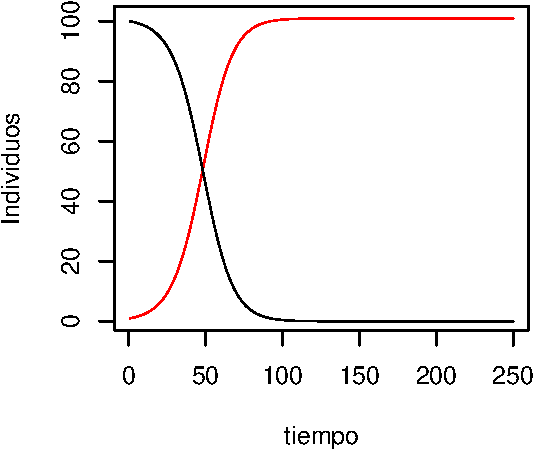
\includegraphics{Modelos-SI-SIR_files/figure-beamer/unnamed-chunk-2-1} 

}

\caption{La línea roja representa el número de infectados, y la negra el de susceptibles.}\label{fig:unnamed-chunk-2}
\end{figure}
\end{frame}

\hypertarget{el-modelo-si-y-levins}{%
\subsection{El modelo SI y Levins}\label{el-modelo-si-y-levins}}

\begin{frame}{El modelo SI y Levins}
\begin{itemize}
\item
  El modelo \(SI\) es equivalente al de metapoblaciones de Levins, donde
  individuos son los parches de hábitat
\item
  Demostración: si \(N = S + I\), y dividimos todo entre \(N\),
  \(s + i = 1\) y \(s = 1-i\)
\item
  Sustituyendo en la ecuación para \(I\), tenemos:
\end{itemize}

\[\frac{di}{dt} = \beta i (1-i)\]
\end{frame}

\hypertarget{el-modelo-sir}{%
\section{\texorpdfstring{El modelo
\(SIR\)}{El modelo SIR}}\label{el-modelo-sir}}

\hypertarget{quuxe9-representa}{%
\subsection{Qué representa}\label{quuxe9-representa}}

\begin{frame}{Qué representa}
Hay tres estados:

Susceptible \(\rightarrow\) Infectado \(\rightarrow\) Recuperado

Por lo tanto hay tres ecuaciones:

\begin{align}
\frac{dS}{dt} &= -\beta SI \\
\frac{dI}{dt} &= \beta SI - \gamma I \\
\frac{dR}{dt} &= \gamma I
\end{align}
\end{frame}

\hypertarget{paruxe1metros-y-estado-de-equilibrio}{%
\subsection{Parámetros y estado de
equilibrio}\label{paruxe1metros-y-estado-de-equilibrio}}

\begin{frame}{Parámetros y estado de equilibrio}
\begin{itemize}
\item
  \(\beta\) es la tasa de transmisión
\item
  \(\gamma\), la tasa de recuperación, ó inverso del tiempo de duración
  de la infección
\item
  El estado de equilibrio también lo encontramos resolviendo para \(I\):
\end{itemize}

\[\beta SI - \gamma I = 0\]

\[I^* = \frac{\beta S}{\gamma}\]
\end{frame}

\hypertarget{el-concepto-r_0}{%
\subsection{\texorpdfstring{El concepto
\(R_0\)}{El concepto R\_0}}\label{el-concepto-r_0}}

\begin{frame}{El concepto \(R_0\)}
\begin{itemize}
\item
  Equilibrio en \(SIR\) es muy diferente de \(SI\)
\item
  Al inicio de una epidemia \(I \approx 1\), por lo que cuando:
\end{itemize}

\[I^* = \frac{\beta S}{\gamma} = 1\]

Se conoce como el umbral \(R_0\), y resolviendo para \(S\), tenemos:

\[S = \gamma/\beta\]
\end{frame}

\hypertarget{quuxe9-representa-s-gammabeta}{%
\section{\texorpdfstring{¿Qué representa
\(S = \gamma/\beta\)?}{¿Qué representa S = \textbackslash gamma/\textbackslash beta?}}\label{quuxe9-representa-s-gammabeta}}

\hypertarget{r_0}{%
\subsection{\texorpdfstring{\(R_0\)}{R\_0}}\label{r_0}}

\begin{frame}{\(R_0\)}
\begin{itemize}
\item
  El tamaño crítico de la comunidad

  \begin{itemize}
  \item
    Densidad poblacional debajo de la cual la epidemia no puede crecer
  \item
    Si \(S < \gamma / \beta\) la infección se extingue
  \end{itemize}
\item
  Si calculamos \(\beta\) y \(\gamma\) para una comunidad con tamaño
  poblacional definido:
\end{itemize}

\[R_0 = \frac{\beta S}{\gamma}\]

\begin{itemize}
\item
  \(R_0\) sólo tiene sentido al inicio de la epidemia
\item
  En ese estado, representa el número de casos secundarios que genera
  cada infectado

  \begin{itemize}
  \tightlist
  \item
    Si \(R_0 > 1\), la epidemia crece, si \(R_0 < 1\) no habrá epidemia
  \end{itemize}
\end{itemize}
\end{frame}

\hypertarget{modelo-sir-con-mortalidad-en-infectados}{%
\subsection{Modelo SIR con mortalidad en
infectados}\label{modelo-sir-con-mortalidad-en-infectados}}

\begin{frame}{Modelo SIR con mortalidad en infectados}
\begin{itemize}
\item
  Caso revisado hasta ahora, no hay efecto de infección sobre
  supervivencia
\item
  Infecciones causan mortalidad, por lo que puede ser necesario
  contemplarla mediante \(\alpha\):
\end{itemize}

\begin{align}
\frac{dS}{dt} &= -\beta SI \\
\frac{dI}{dt} &= \beta SI - (\gamma + \alpha) I \\
\frac{dR}{dt} &= \gamma I
\end{align}
\end{frame}

\hypertarget{esquema-el-modelo-sir-con-mortalidad}{%
\subsection{\texorpdfstring{Esquema el modelo \(SIR\) con
mortalidad}{Esquema el modelo SIR con mortalidad}}\label{esquema-el-modelo-sir-con-mortalidad}}

\begin{frame}{Esquema el modelo \(SIR\) con mortalidad}
\href{Esquemas-SIR.pdf}{Esquema}
\end{frame}

\hypertarget{modelos-de-transmisiuxf3n-frecuento-dependiente}{%
\section{Modelos de transmisión
frecuento-dependiente}\label{modelos-de-transmisiuxf3n-frecuento-dependiente}}

\hypertarget{intro}{%
\subsection{Intro}\label{intro}}

\begin{frame}{Intro}
\begin{itemize}
\item
  Denso-dependencia se basa en densidad crítica de permite transmisión
\item
  Frecuento-dependencia, no requiere densidad mínima

  \begin{itemize}
  \tightlist
  \item
    Representa enfermedades con dinámicas de transmisión más lenta
  \end{itemize}
\end{itemize}

Denso-dependencia, ó acción de pseudo-masas:

\[\beta SI\]

Frecuento-dependencia:

\[\beta S \frac{I}{N}\]

donde \(I/N\) es \ldots{}
\end{frame}

\hypertarget{section}{%
\subsection{\ldots{}}\label{section}}

\begin{frame}{\ldots{}}
La prevalencia de la infección
\end{frame}

\hypertarget{el-modelo-sir-con-transmisiuxf3n-frecuento-dependiente}{%
\subsection{El modelo SIR con transmisión
frecuento-dependiente}\label{el-modelo-sir-con-transmisiuxf3n-frecuento-dependiente}}

\begin{frame}{El modelo SIR con transmisión frecuento-dependiente}
\begin{align}
\frac{dS}{dt} &= - \beta S \frac{I}{N} \\
\frac{dI}{dt} &= \beta S \frac{I}{N} - \gamma I \\
\frac{dR}{dt} &= \gamma I
\end{align}

A este modelo se pueden añadir términos igual que al denso-dependiente
\end{frame}

\hypertarget{condiciones-de-estabilidad}{%
\subsection{Condiciones de
estabilidad}\label{condiciones-de-estabilidad}}

\begin{frame}{Condiciones de estabilidad}
Derivemos la expresión para \(R_0\), tomando en cuenta que \(N = S+I\):

\begin{enumerate}
\item
  \(\beta - \gamma I = 0\)
\item
  \(\beta \frac{SI}{S+I} = \gamma(S+I)\)
\item
  Debido que al inicio de la epidemia \(S \approx N\):
\end{enumerate}

\[\beta I = \gamma I \rightarrow \frac{\beta}{\gamma} = 1\]

Las condiciones que evitarían la epidemia dependen de \(\beta\) y
\(\gamma\), no de \(S\)
\end{frame}

\hypertarget{caos-en-el-modelo-sir}{%
\section{Caos en el modelo SIR}\label{caos-en-el-modelo-sir}}

\hypertarget{eliminando-la-dimensionalidad-del-modelo}{%
\subsection{Eliminando la dimensionalidad del
modelo}\label{eliminando-la-dimensionalidad-del-modelo}}

\begin{frame}{Eliminando la dimensionalidad del modelo}
\begin{itemize}
\tightlist
\item
  Transformar tamaños poblacionales en proporciones, con base en:
\end{itemize}

\begin{align}
N & = S+I+R \\
s & = S/N \\
i & = I/N \\
r & = R/N \\
n & = 1 = N/N
\end{align}
\end{frame}

\hypertarget{el-sistema-de-ecuaciones}{%
\subsection{El sistema de ecuaciones}\label{el-sistema-de-ecuaciones}}

\begin{frame}{El sistema de ecuaciones}
\begin{align}
\frac{ds}{dt} & = n  - \beta si - \mu s\\
\frac{di}{dt} & = \beta si - (\gamma + \alpha + \mu) i \\
\frac{dr}{dt} & = \gamma i - \mu r
\end{align}
\end{frame}

\hypertarget{la-funciuxf3n-de-desolve}{%
\subsection{\texorpdfstring{La función de
\texttt{deSolve}}{La función de deSolve}}\label{la-funciuxf3n-de-desolve}}

\begin{frame}[fragile]{La función de \texttt{deSolve}}
\begin{Shaded}
\begin{Highlighting}[]
\NormalTok{sir }\OtherTok{\textless{}{-}} \ControlFlowTok{function}\NormalTok{(t, y, parms)\{}
\NormalTok{  s }\OtherTok{\textless{}{-}}\NormalTok{ y[}\DecValTok{1}\NormalTok{]}
\NormalTok{  i }\OtherTok{\textless{}{-}}\NormalTok{ y[}\DecValTok{2}\NormalTok{]}
\NormalTok{  r }\OtherTok{\textless{}{-}}\NormalTok{ y[}\DecValTok{3}\NormalTok{]}
  \FunctionTok{with}\NormalTok{(parms,}
\NormalTok{       \{}
\NormalTok{         ds }\OtherTok{\textless{}{-}}\NormalTok{ n }\SpecialCharTok{*}\NormalTok{ s }\SpecialCharTok{{-}}\NormalTok{ beta }\SpecialCharTok{*}\NormalTok{ s }\SpecialCharTok{*}\NormalTok{ i }\SpecialCharTok{{-}}\NormalTok{ mu }\SpecialCharTok{*}\NormalTok{ s}
\NormalTok{         di }\OtherTok{\textless{}{-}}\NormalTok{ beta }\SpecialCharTok{*}\NormalTok{ s }\SpecialCharTok{*}\NormalTok{ i }\SpecialCharTok{{-}}\NormalTok{ (alfa }\SpecialCharTok{+}\NormalTok{ mu }\SpecialCharTok{+}\NormalTok{ gamma) }\SpecialCharTok{*}\NormalTok{ i}
\NormalTok{         dr }\OtherTok{\textless{}{-}}\NormalTok{ gamma }\SpecialCharTok{*}\NormalTok{ i  }\SpecialCharTok{{-}}\NormalTok{ mu }\SpecialCharTok{*}\NormalTok{ r}
         
         \FunctionTok{return}\NormalTok{(}\FunctionTok{list}\NormalTok{(}\FunctionTok{c}\NormalTok{(ds, di, dr)))}
\NormalTok{       \})}
\NormalTok{\}}
\end{Highlighting}
\end{Shaded}
\end{frame}

\hypertarget{las-dinuxe1micas-oscilatorias-de-sir}{%
\subsection{\texorpdfstring{Las dinámicas oscilatorias de
\(SIR\)}{Las dinámicas oscilatorias de SIR}}\label{las-dinuxe1micas-oscilatorias-de-sir}}

\begin{frame}{Las dinámicas oscilatorias de \(SIR\)}
\begin{center}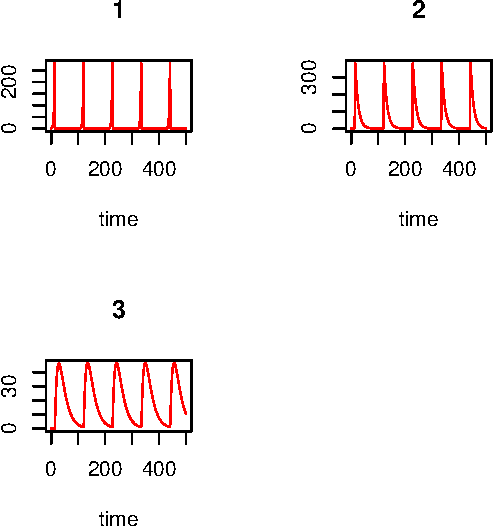
\includegraphics{Modelos-SI-SIR_files/figure-beamer/unnamed-chunk-5-1} \end{center}
\end{frame}

\end{document}
